\documentclass[11pt,a4paper]{article}
\usepackage{natbib}
\usepackage{fullpage}
\usepackage{draftwatermark}
\SetWatermarkText{DRAFT}
\SetWatermarkScale{5}
\title{\textbf{Clinician's challenge entry}}
\author{GR, AJG, RM}
		\date{\today}

\usepackage{graphicx}
\begin{document}
\maketitle

\section{Introduction}

This paper describes the development, implementation, and evaluation  of an autonomous decision support tool for the interpretation of renal function tests. The tool provides clinicians with suggestions about the further management of a patient's test results. These suggestions are designed to be patient and context specific. The motivations behind the development of this application were to improve the quality of care patients experience, and to support the General Practitioner teams to manage the volume of results they receive on a daily basis. \\

An example was the discovery of an instance of an abnormal renal function result in a patient who was acutely unwell. An experienced and caring physician had reviewed the latest renal function test result, making a clinical entry indicating the result was normal. This interpretation of the result did not seem to include the clinical context in which the test was requested or the patient's previous renal function test results. Despite the result being highly significant, the report did not generate any action until the patient re-presented several weeks later, still feeling unwell. Fortunately, this case ended well for the patient.\\

For any patient, this is concerning but not uncommon. One study reported that American primary care physicians spent 74 minutes per day reviewing results. Despite which 81\% reported delays in managing results and only 41\% of clinicians were satisfied with their current process \citep{poon2004wish}. Estimates of "missed" or not followed up results vary from 6.8\% to 62\% \citep{callen2012failure}.\\

Another motivation was the rising incidence of chronic renal disease and the associated costs to society. The estimated Canadian prevalence of chronic renal disease in 2007-2009 was 12.5\% and 3.1\% of the population has grade 3-5 disease \citep{arora2013prevalence}. \citep{anachronistic}, described how despite the rising significance of renal disease worldwide, practitioner awareness remains low. These authors argued that care would need to be led by primary care and integrated into general chronic condition management to avoid the "catastrophic" costs associated with the management of advanced chronic renal disease management \citep{jha2013chronic}. Kerr et al. estimated the cost of renal disease at 1.44-1-45 billion Pound Stirling in 2009-2010 for the UK alone \citep{underestimating}.\\

\section{Method}
Ensuring patient safety at all times drove all design decisions in the development of RenalQ. Therefore, the clinician was to remain responsible for the final determination of further care of the patient.   The decision for the clinician to be the final arbitrator also acknowledges the possibility of error with an application like RenalQ during its development phase. \\

The decision was also made to adopt modern production methodology which has used statistical process control (SPC) as part of "production business management" \citep{rosemann2015six, cheng2015run, epprecht2015statistical}. Adoption of SPC enabled RenalQ to function at the necessary scale to operate within a DHB's laboratory services, and also to  be able to consider the individual patient's needs. In health SPC has already been used to study the operational function of emergency departments \citep{pimentel2015statistical} and the widest adoption of SPC in health has been within the field of quality improvement \citep{provost2011health}.\\

The technical description of the application and its development is more fully described elsewhere \citep{GodfreyEtAl2014KidneyPaper}. In essence, RenalQ interprets the estimated Glomerular Filtration Rate (eGFR) result for each patient, within the context of their previous eGFR results. In the laboratory workflows, RenalQ is executed after the usual renal function tests. In any circumstances where it is inappropriate for the eGFR not to be calculated, RenalQ is not executed, such as for pregnant women or children. \\

The RenalQ interpretation engine consists of three layers depending on the number of eGFR results available within the laboratory database. If there are less than five results available, no specific advice is given by RenalQ. If there are five to nineteen  results available, the context of the latest eGFR result is interpreted by a set of fixed heuristic rules which encode current standard clinical practice. As a safeguard, any result returned by the application to the treating clinician would be clinically conservative, thus encouraging the  clinician to be proactive in their care of the patient. Patient safety was prioritized, but this meant accepting RenalQ might occasionally be unnecessarily alarmist in its interpretations. Additional rules were established to ensure that a wide range of possible eGFR patterns were being handled appropriately.  One such rule was necessary for RenalQ to reliably detect acute renal failure. The third layer in the RenalQ interpretation engine was for patients where twenty  or more test results were available for SPC to provide an analysis. This third layer used control chart methodology, notably including a cumulative summation procedure to determine changes between the current eGFR result and previous results. From this result, RenalQ develops recommendations for the clinician.  

Considerable work was required to integrate the RenalQ' application into the laboratory systems before the pilot study of its functionality in clinical practice.  The technical complexities were in transferring data between the laboratory systems and RenalQ,  and then for the analysis results to be returned to the Laboratory systems.  The returned RenalQ results were then integrated into the standard renal function test results for return to the clinician, and retention in the patient's clinical records. \\

Once the application was operationally ready for evaluation by primary care, ethical approval for the trial to proceed was then gained from the MidCentral and Central PHO clinical boards. \\

\section{Evaluation}
Pre-deployment the focus of evaluation was on the optimization of the interpretation engine using a series of progressively larger cohorts of deidentified historic renal function results. \\

Once the algorithm was optimized, sensitivity was over 99\% specificity was over 98\%.  As a safeguard, the results of RenalQ were reviewed by the local renal physicians to ensure selectivity and specificity were progressively optimised. As a group, they were comfortable with the interpretations provided by RenalQ as being safe and appropriate for a pilot study. As part of the pilot studies, RenalQ was evaluated qualitatively and quantitatively. \\

\subsection{Qualitative results}
A semi-structured interview instrument was selected as it allowed primary care staff to both reflect on their experiences with RenalQ and enabled them to provide in-depth feedback. In the "responsive interview" method, the emphasis is on the fact that the interviewer and interviewee are both people and that they form a relationship during the interview \citep{rubin2011qualitative}. Additionally, this method allows the research design to remain flexible meaning that if new information, or a new area of interest, is uncovered then the current interview, and subsequent interviews, can probe this area. \\

A series of interviews of individual clinicians and groups were undertaken. Where interviews were conducted, the semi structured responsive interview process was followed. Where a large group was encountered the approach was altered into a focus group approach based on the semi-structured questions.\\

Validity in qualitative research is seen as an activity that is conducted throughout the research process \citep{morse2002verification, kvale2009interviews} to convince readers of the likelihood that the support for the claim is strong enough to serve as a basis for understanding \citep{polkinghorne2007validity}. Throughout the qualitative process it was the views of primary care staff that were sought, listened to, and clarified where meaning was not understood. The result of the process is that the research reflects the primary care view of RenalQ and not that of the researcher.\\

At each interview or focus group there was a clear message that RenalQ added value to general practice. Reflective comments from General Practitioners included - “don’t take it away” and a “really useful tool”. The General Practitioners interviewed appeared to place confidence on the RenalQ interpretation and they reflected that this both “sharpened their practice” and “saved time”.\\

The reflection of General Practitioners that RenalQ was felt to save time was in contrast with what was originally considered that it would increase General Practitioner workload. The General Practitioner perspective on this aspect was that the RenalQ interpretation provided an additional check giving them confidence in their proposed action. In part this was due to the believe that the sensitivity of RenalQ with respect to its interpretations was set conservatively and this was considered appropriate.\\

In addition General Practitioners felt the RenalQ process could be applied to outpatient renal function tests from the hospital in addition to community requested samples. This anomaly is due the laboratory deeming all hospital samples to be taken from patients not in their steady state, not just those acutely unwell. General Practitioners also considered the statistical processes could be extended to other areas of laboratory result interpretation. \\

\subsection{Quantitative results}
On release of RenalQ into district wide pilot, utilization data became available. The principle measures analysised where the frequency of testing and the elapsed time to the next test against the eGFR result.\\

In the following analysis, the data for 2013 has been added back in and we have evaluated every value of eGFR instead of grouped eGFR values. The next  model  used to identify the statistically significant factors affecting the time between successive renal function tests allows for only the level of renal function for each patient (as measured by their eGFR), and whether that test was analyzed using the RenalQ system. In addition, the combination of these two effects has also been incorporated in the model. The regression model for this model yields  the following summary of effects and their statistical significance. These show that there has been a statistically significant reduction in the time of next test for patients with serious renal impairment; a logrithmic scale is required to visualise the effect due to the differing magnitudes for the grouped data.\\

\begin{figure}[htp]
\centering
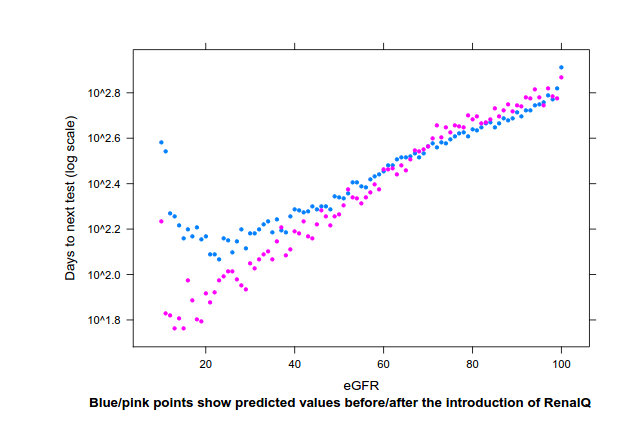
\includegraphics[scale=0.50]{FigCritical.png}
\caption{}
\label{}
\end{figure}

The pattern of change in time to next test is in accordance with our projections. We were expected the result of a decrease between tests for patients with serious renal impairment. The middle zone of mild renal impairment fulfilled our expectation of no change. Only time will tell if the expected increase in time between tests for those patients with mild or no renal impairment occurs. Given the time between tests in this group of patients is expected to be measured in years, it will be some time before our hypothesis is confirmed. The clinical benefit of RenalQ is already established through the reduction or optimisation between tests for those patients with moderate to severe renal impairment. Any financial benefit will only occur with reduction in testing frequency in those with mild or no renal impairment.

\pagebreak

\bibliographystyle{plain}
\bibliography{NZMJ}

\end{document}